\documentclass[14pt,a4paper,report]{report}
\usepackage[a4paper, mag=1000, left=2.5cm, right=1cm, top=2cm, bottom=2cm, headsep=0.7cm, footskip=1cm]{geometry}
\usepackage[utf8]{inputenc}
\usepackage[english,russian]{babel}
\usepackage{indentfirst}
\usepackage[dvipsnames]{xcolor}
\usepackage[colorlinks]{hyperref}
\usepackage{listings} 
\usepackage{fancyhdr}
\usepackage{caption}
\usepackage{amsmath}
\usepackage{latexsym}
\usepackage{graphicx}
\usepackage{amsmath}
\usepackage{booktabs}
\usepackage{array}
\hypersetup{
	colorlinks = true,
	linkcolor  = black
}

\usepackage{titlesec}
\titleformat{\chapter}
{\Large\bfseries} % format
{}                % label
{0pt}             % sep
{\huge}           % before-code


\DeclareCaptionFont{white}{\color{white}} 

% Listing description
\usepackage{listings} 
\DeclareCaptionFormat{listing}{\colorbox{gray}{\parbox{\textwidth}{#1#2#3}}}
\captionsetup[lstlisting]{format=listing,labelfont=white,textfont=white}
\lstset{ 
	% Listing settings
	inputencoding = utf8,			
	extendedchars = \true, 
	keepspaces = true, 			  	 % Поддержка кириллицы и пробелов в комментариях
	language = Matlab,            	 	 % Язык программирования (для подсветки)
	basicstyle = \small\sffamily, 	 % Размер и начертание шрифта для подсветки кода
	numbers = left,               	 % Где поставить нумерацию строк (слева\справа)
	numberstyle = \tiny,          	 % Размер шрифта для номеров строк
	stepnumber = 1,               	 % Размер шага между двумя номерами строк
	numbersep = 5pt,              	 % Как далеко отстоят номера строк от подсвечиваемого кода
	backgroundcolor = \color{white}, % Цвет фона подсветки - используем \usepackage{color}
	showspaces = false,           	 % Показывать или нет пробелы специальными отступами
	showstringspaces = false,    	 % Показывать или нет пробелы в строках
	showtabs = false,           	 % Показывать или нет табуляцию в строках
	frame = single,              	 % Рисовать рамку вокруг кода
	tabsize = 2,                  	 % Размер табуляции по умолчанию равен 2 пробелам
	captionpos = t,             	 % Позиция заголовка вверху [t] или внизу [b] 
	breaklines = true,           	 % Автоматически переносить строки (да\нет)
	breakatwhitespace = false,   	 % Переносить строки только если есть пробел
	escapeinside = {\%*}{*)}      	 % Если нужно добавить комментарии в коде
}

\begin{document}

\def\contentsname{Содержание}

% Titlepage
\begin{titlepage}
	\begin{center}
		\textsc{Санкт-Петербургский Политехнический 
			Университет Петра Великого\\[5mm]
			Кафедра компьютерных систем и программных технологий}
		
		\vfill
		
		\textbf{Отчёт по лабораторной рабте №4\\[3mm]
			Курс: «Методы оптимизации и принятия решений»\\[3mm]
			Тема: «Оптимизация систем массового обслуживания»\\[35mm]
			}
	\end{center}
	
	\hfill
	\begin{minipage}{.5\textwidth}
		Выполнил студент:\\[2mm] 
		Ерниязов Тимур Ертлеуевич\\
		Группа: 13541/2\\[5mm]
		
		Проверил:\\[2mm] 
		Сиднев Александр Георгиевич
	\end{minipage}
	\vfill
	\begin{center}
		Санкт-Петербург\\ \the\year\ г.
	\end{center}
\end{titlepage}

% Contents
\tableofcontents
\clearpage

\chapter{Лабораторная работ №4}

\section{Индивидуальное задание}

Рассмотрите идеализированную сеть связи с N=4 узлами, для которой справедлива простая модель с M/M/1. Предполагается, что μ=1, а матрица трафика ($Y_{ij}$) и матрица маршрутов ($r_{ij}$) (где $r_{ij}$ – номер следующего узла, в который должно быть передано сообщение, если сейчас оно находится в узле j и окончательно адресовано узлу i) имеют вид:


$$Y_{jk} = 
\begin{bmatrix} 
0 & 2 & 1 & 2 \\
1 & 0 & 1 & 1 \\
4 & 1 & 0 & 1 \\
1 & 1 & 0 & 0 \\
\end{bmatrix}
\quad 
r_{ij} = 
\begin{bmatrix} 
- & 2 & 1 & 3 \\
2 & - & 1 & 3 \\
2 & 4 & - & 3 \\
2 & 4 & 1 & - \\
\end{bmatrix}
\quad $$


\begin{enumerate}
    \item Найдите среднюю длину пути.
        \item Пусть задана полная пропускная способность C = 34. Найдите пропускные способности {C_i}, которые минимизируют среднюю задержку сообщения T. Если для С=34, не выполняются условия наличия установившегося режима, то следует самостоятельно увеличить С с тем, чтобы указанные условия выполнялись.
            \item 	Изобразите сеть, снабдите каждое ребро стрелкой и парой (λ_i,C_i).

                \item 	Найдите T.

                    \item Определите «длины каналов» с использованием формулы (5.40) из книги Л. Клейнрока «ВС с очередями». Найдите все кратчайшие маршруты из узла в узел, используя один из следующих подходов:
                    
                    \begin{itemize}
    \item 	применение алгоритма Флойда, дополненного процедурой сбора и правильной расстановки транзитных узлов;

        \item 	применение алгоритма перечисления путей из узла в узел, предполагающего возведение в степень булевой примитивной матрицы

            \item 	применение любого другого алгоритма, решающего эту же задачу с кратким пояснением и указанием источника.

\end{itemize}
                    
                    
                    
                        \item 	Пусть сделан пропорциональный выбор пропускных способностей. Найдите {Ci} и T и проведите сравнение с результатом пункта Г. Пропорциональный выбор пропускных способностей 

\end{enumerate}





\clearpage


\section{Ход работы}
\subsection{Расчет длины путей}
С помощью таблицы маршрутов найдем транзитные узлы для каждого из маршрутов

$$Y_{jk} = 
\begin{bmatrix} 
0 & 2 & 1 & 2 \\
1 & 0 & 1 & 1 \\
4 & 1 & 0 & 1 \\
1 & 1 & 0 & 0 \\
\end{bmatrix}
\quad 
r_{ij} = 
\begin{bmatrix} 
- & 2 & 1 & 3 \\
2 & - & 1 & 3 \\
2 & 4 & - & 3 \\
2 & 4 & 1 & - \\
\end{bmatrix}
\quad $$


\begin{table}[h!]
\begin{tabular}{|l|l|l|l|}
\hline
 Начало & Промежуточный маршрут & Конец   \\ \hline
1 & - & 2 \\ \hline
1 & 24 & 3 \\ \hline
1 & 2 & 4 \\ \hline
2 & 43 & 1 \\ \hline
2 & 4 & 3 \\ \hline
2 & - & 4 \\ \hline
3 & - & 1 \\ \hline
3 & 1 & 2 \\ \hline
3 & 12 & 4 \\ \hline
4 & 3 & 1 \\ \hline
4 & 31 & 2 \\ \hline
4 & - & 3 \\ \hline
\end{tabular}%
\end{table}

Обозначим каналы и запишем значение интенсивностей их потоков:

\begin{enumerate}
    \item $y_{12} = y_{13} + y_{14} +  y_{34} +  y_{32}  + y_{42} = 6$
    \item $y_{24} = y_{13} + y_{14} +  y_{21}  + y_{23}  + y_{34} = 6$
    \item $y_{31} = y_{21} + y_{32} +  y_{34}  + y_{41} +  y_{42} = 5$
    \item $y_{43} = y_{13} + y_{21}  + y_{23}  + y_{41} +  y_{42} = 5$
\end{enumerate}


Полный внешний трафик, поступающий в сеть:
$$ Y = \sum_{j=1}^N  \sum_{k=1}^N Y_{jk} =16 $$

Полный трафик в сети:
$$ \lambda = \sum_{i=1}^M = \sum_{j=1}^N  \sum_{k=1}^N Y_{jk} = 22 $$

Средняя длина пути:
$$ n = \frac{\lambda}{Y} =\frac{22}{16} = 1.3750
  $$




\subsection{Задача выбора пропускных способностей}


Дано: потоки ${\lambda_i}$ и топология сети
Минимизировать $T$.
Варьируются: ${C_i}$.
Ограничение:
$$ D= \sum_{i=1}^M d_i (C_i)$$
, где $d_i(C_i)$ – стоимости каналов. В качестве стоимости каналов возьмем их пропускные способности.

$$ C_i = \frac{\lambda_i}{\mu} + C(1-n p) \frac{\sqrt{\lambda_i}}{ \sum_{j=1}^M \sqrt{\lambda}},  i=1,2,… M$$ 



$C = \begin{pmatrix} 
9.1366 \\
9.1366 \\
7.8634 \\
7.8634 
\end{pmatrix}
\quad$



Схема сети, представлена на Рис. 1.1.

\begin{figure}[h!]
\center{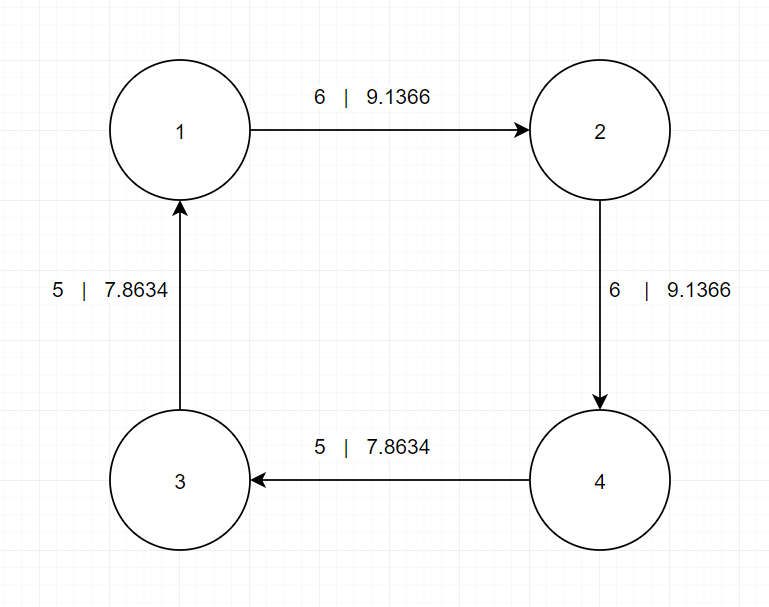
\includegraphics[width=1\linewidth]{sheme}}
\caption{Схема сети}
\label{ris:image}
\end{figure}


Средняя задержка сообщений:
$$ T = \frac{n(\sum_{i=1}^M \sqrt{\lambda_i⁄\lambda}  )^2 }{\mu C(1-np)} = 0.4574  $$


Длины каналов:

$$ l_i = \frac{C_i}{Y(C_i- \frac{\lambda_i}{\mu})^2} $$


$$l =
\begin{pmatrix}
0.0580 \\
0.0580 \\
0.0599 \\
0.0599
\end{pmatrix}
\quad
$$ 

\subsection{Нахождение длины кратчайших маршрутов с использованием алгоритма Флойда}

Используем алгоритм Флойда для вычисления кратчайших маршрутов, который описан в скрипте Matlab. 

Результаты вычислений:

$$ D = \begin{bmatrix}  
0 & 9.1366 & 26.1366 & 18.2732 \\
24.8634 & 0 & 17 & 9.1366 \\
7.8634 & 17 & 0 & 26.1366 \\
15.7268 & 24.8634 & 7.8634 & 0 
\end{bmatrix}
P=\begin{bmatrix} 
[     ] & [2    ] & [2 4 3] & [2 4  ] \\
[4 3 1] & [2    ] & [4 3  ] & [4    ] \\
[1    ] & [1 2  ] & [     ] & [1 2 4] \\
[3 1  ] & [3 1 2] & [3    ] & [     ] \end{bmatrix}$$

Матрица D содержит длины маршрутов. Матрица P - пути


\subsection{Пропорциональный выбор пропускных способностей}

Так как трафик в последнем канале отсутствует и интенсивность нулевая, можно исключить его из системы, иначе задержка становится равной бесконечности




$$ C_i = \frac{\lambda_i}{\lambda}*C $$



$C = \begin{pmatrix} 
9.2727 \\
9.2727 \\
7.7273 \\
7.7273
\end{pmatrix}
\quad$



$$ T = \sum_{i=1}^M* \frac{\lambda_i}{Y} \frac{1}{\mu C_i-\lambda_i }=0.4583  $$















Все расчеты проводились в Matlab:
\begin{lstlisting}[language={matlab}, caption={Скрипт}, basicstyle=\ttfamily]
clc;
y = [0 2 1 2; 1 0 1 1; 4 1 0 1; 1 1 0 0]; % матрица трафика
n = [0 2 1 3; 2 0 1 3; 2 4 0 3; 2 4 1 0]; % матрица маршрутов
C = 34; % полная пропускная способность
u = 1;

coef_p = ((sum(sum(y)))*u/C); % коэффициент загрузки (отношение внешнего траффика в битах от суммарной пропускной способности)

% Интенсивности потока
L_i = [(y(1,3)+y(1,4)+y(3,2)+y(4,2)+y(3,4));
    (y(1,3)+y(1,4)+y(2,1)+y(2,3)+y(3,4));
    (y(2,1)+y(3,2)+y(3,4)+y(4,1)+y(4,2));
    (y(1,3)+y(2,1)+y(2,3)+y(4,1)+y(4,2))];

Y = sum(sum(y)); % внешний трафик поступающий в сеть
lam = sum (sum (L_i)); % полный трафик в сети
n_ = lam/Y; % средняя длина пути


% Задача выбора пропускных способностей
C_i = L_i + C*(1-n_*coef_p)*((L_i.^0.5)/sum(L_i.^0.5));
% Оптимальное значение задержки
T = n_*(sum((L_i/(sum(L_i))).^0.5)^2)/(C*u*(1-n_*coef_p));

% Ддины каналов
l_i = C_i./(Y*(C_i - L_i).^2);


%% Нахождение кратчайших маршрутов из узла в узел с использованием алгоритма Флойда
R = [Inf   2   1   3;
       2 Inf   1   3;
       2   4 Inf   3;
       2   4   1 Inf];
   
D = [  0 Inf Inf Inf;
     Inf   0 Inf Inf;
     Inf Inf   0 Inf;
     Inf Inf Inf   0];
 
% Траектории 
p = cell(4);

for i = 1:4
    for j = 1:4
        b = R(i, j);
        if b ~= Inf
            D(j, b) = 1;
            p{j, b} = [b];
        end
    end 
end

for k = 1:4
    for i = 1:4
        for j = 1:4
            new_d = D(i, k) + D(k, j);  
            if new_d < D(i, j)
                D(i, j) = new_d;
                p{i, j} = [p{i, k}, p{k, j}];   
            end
        end
     end
end

% Алгоритм флойда
D = [  0       9.1366  Inf     Inf;
       Inf     0  Inf     9.1366;
       7.8634  Inf     0       Inf ;
       Inf     Inf     7.8634  0;];
   
prevD = D;
 
for k = 1:length(D)
  D = min(D,D(:,k) + D(k,:));
  prevD = D;
end
    
% Пропускные способности для случая пропорционального выбора 
C_i_proporz = (L_i/lam)*C;
% Средняя задержка для случая пропорционального выбора
T_proporz = sum((L_i/Y./(C_i_proporz-L_i)));

%% Форматированый вывод
fprintf('Коэффициент загрузки: %4.4f \n',coef_p)
fprintf('Интенсивности потока:\n')
fprintf('%d\n', L_i)
fprintf('Внешний трафик поступающий в сеть: %4.4f \n',Y);
fprintf('Полный трафик в сети: %4.4f \n',lam)
fprintf('Cредняя длина пути: %4.4f \n',n_)
fprintf('Пропускные способности:\n')
fprintf('%4.4f\n', C_i)
fprintf('Оптимальное значение задержки: %4.4f \n',T)
fprintf('Ддины каналов:\n')
fprintf('%4.4f\n',l_i)
fprintf('Матрица длин маршрутов:\n')
fprintf('%4.4f %4.4f %4.4f %4.4f \n', D.')
fprintf('Матрица с путем:\n')
for ii = 1:4
    for jj = 1:4
        pp = p{ii, jj};
        fprintf('[');
        for k = 1:3
            if k <= size(pp, 2)
                fprintf('%d', pp(k));
            else
                fprintf(' ');
            end
            if k < 3
                fprintf(' ');
            end
        end
        fprintf('] ');
    end
    fprintf('\n');
end    
fprintf('Пропускные способности для случая пропорционального выбора :\n')
fprintf('%4.4f\n', C_i_proporz)
fprintf('Оптимальное значение задержки для случая пропорционального выбора : %4.4f \n',T_proporz)
\end{lstlisting}


\begin{lstlisting}[language={matlab}, caption={Резульаты}, basicstyle=\ttfamily]
Коэффициент загрузки: 0.4706 
Интенсивности потока:
6
6
5
5
Внешний трафик поступающий в сеть: 16.0000 
Полный трафик в сети: 22.0000 
Cредняя длина пути: 1.3750 
Пропускные способности:
9.1366
9.1366
7.8634
7.8634
Оптимальное значение задержки: 0.4574 
Ддины каналов:
0.0580
0.0580
0.0599
0.0599
Матрица длин маршрутов:
0.0000 9.1366 26.1366 18.2732 
24.8634 0.0000 17.0000 9.1366 
7.8634 17.0000 0.0000 26.1366 
15.7268 24.8634 7.8634 0.0000 
Матрица с путем:
[     ] [2    ] [2 4 3] [2 4  ] 
[4 3 1] [2    ] [4 3  ] [4    ] 
[1    ] [1 2  ] [     ] [1 2 4] 
[3 1  ] [3 1 2] [3    ] [     ] 
Пропускные способности для случая пропорционального выбора :
9.2727
9.2727
7.7273
7.7273
Оптимальное значение задержки для случая пропорционального выбора : 0.4583 
>> 
\end{lstlisting}


\section{Вывод}

В данной лабораторной работе был рассмотрен пример оптимизации идеализированной системы массового обслуживания.
В ходе работы был произведен расчет средней длины пути, составлена схема сети, а также двумя способами решена задача выбора пропускных способностей.

	Пропорциональное распределение оказалось хуже чем оптимальное, т.к. имеет большую среднюю задержку.



\end{document}